
% !TEX encoding = UTF-8 Unicode 
% !TEX root = FieldGuide.tex

\subpart{One shape parameter}


\Sec{Power Function Distribution}
\label{sec:PowerFn}


\dist{Power function} (power) distribution~\cite{Pearson1916, Meniconi1996,Johnson1995} 
is  a three parameter, continuous, univariate, unimodal probability density, with finite or semi-infinite support. The functional form in most straightforward  parameterization consists of a single power function.
\begin{align}
\label{PowerFn}
\opr{PowerFn}(x\given a,s,\beta) &= 
\left|\frac{\beta}{ s}\right|
\left(\frac{x-a}{s} \right)^{\beta -1} \checked
%\\ &= \opr{GenBeta}(x\given a,s , \alpha,1,1) \notag 
\\
\notag  \text{for } & x, a, s, \beta \text{ in } \mathbb{R}
 \\ \text{ support } & x \in [a,a+s], s>0,\ \beta>0 \notag \checked
  \\ \text{ or } &  x\in[a+s,a], s<0,\ \beta>0  \checked
 \notag 
 \\  \notag  \text{ or } &  x\in[a+s,+\infty], s>0,\ \beta<0 \checked
 \\  \notag  \text{ or } &  x\in[-\infty,a+s], s<0,\ \beta<0 \checked
 \notag
\end{align}
%
%Pearson~\cite{Pearson1916, Johnson1994} noted two special cases, the monotonically decreasing {\bf Pearson type VIII} $0<\beta <1$, and the monotonically increasing {\bf Pearson type IX} distribution~\cite{Pearson1916, Johnson1994} with $\beta>1$. 
With positive $\beta$ we obtain a distribution with finite support. But by allowing $\beta$ to extend to negative numbers, the power function distribution also encompasses the semi-infinite Pareto distribution \eqref{Pareto}, and in the limit $\beta\rightarrow\infty$ the exponential distribution \eqref{Exp}.


\SSec{Alternative parameterizations}

% CITATION NEEDED
\dist{Generalized Pareto} distribution: An alternative parameterization that emphasizes the limit to exponential.
\begin{align}
\label{GenPareto}
\opr{GenPareto}&(x\given a',s',\xi) 
\\ & =
 \begin{cases}
  \frac{1}{|\theta|}\left( 1 + \xi \frac{x-\pLoc}{\theta}\right)^{-\tfrac{1}{\xi}-1} & \xi \neq 0 \checked
\notag
\\ 
 \frac{1}{|\theta|} \exp \left(-\frac{x-\pLoc}{\theta} \right)& \xi = 0 \checked
\notag
\end{cases}
\\
& = \opr{PowerFn}(x\given \pLoc-\tfrac{\theta}{\xi},\tfrac{\theta}{\xi},  -\tfrac{1}{\xi}) \checked
\notag
\end{align}


% CITATION NEEDED
\dist{q-exponential} (generalized Pareto) distribution is an alternative parameterization of the power function distribution, utilizing the Tsallis generalized q-exponential function, $\exp_q(x)$ \secref{sec:Limits}.
\begin{align}
\label{QExp}
\opr{QExp}&(x\given  \pLoc,\theta,q) \\
\notag
= & \frac{(2-q)}{|\theta|} \exp_q\left(- \frac{x-\pLoc}{\theta} \right)  \checked
\\  
= &
\begin{cases}
\frac{(2-q)}{|\theta|}\left(1 - (1-q) \frac{x-\pLoc}{\theta} \right)^{\frac{1}{1-q}} & q \neq 1 \checked
\\
\notag
\tfrac{1}{|\theta| }\exp\left(- \frac{x-\pLoc}{\theta} \right)  & q=1 \checked
\end{cases}
\notag
\\
=&  \opr{PowerFn}(x\given \pLoc+\frac{\theta}{1-q},-\frac{\theta}{1-q},\frac{2-q}{1-q}) \checked
\\
\notag  \text{for } & x, \pLoc, \theta, q \text{ in } \mathbb{R}
\end{align}



\begin{figure}[p]
\begin{center}
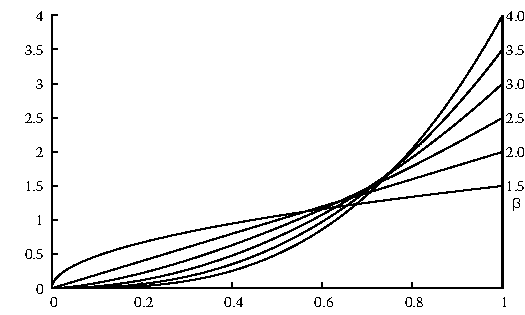
\includegraphics[width=\textwidth]{pdfPowerFn}
\end{center}
\caption[Pearson IX distributions]{Pearson type IX, $\opr{PowerFn}(x\given 0,1,\beta)$, $\beta>1$
}
\end{figure}
%
%
\begin{figure}[p]
\begin{center}
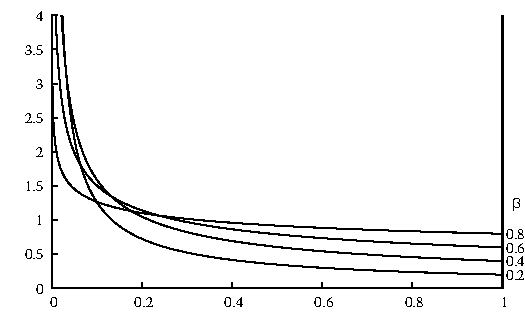
\includegraphics[width=\textwidth]{pdfPowerFn2}
\end{center}
\caption[Pearson VIII distributions]{Pearson type VIII, $\opr{PowerFn}(x\given 0,1,\beta)$, $0<\beta<1$. }
\end{figure}
%
\begin{figure}[tp]
\begin{center}
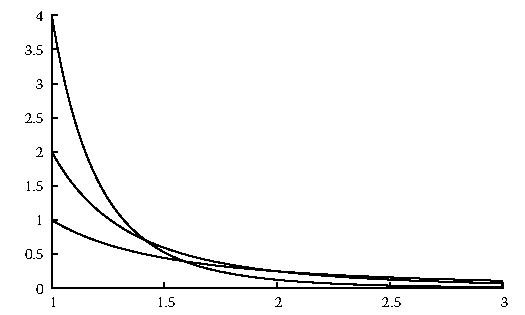
\includegraphics[width=\textwidth]{pdfPareto}
\end{center}
\caption[Pareto distributions]{Pareto distributions, $\opr{Pareto}(x\given 0,1,\bar\beta)$, $\bar\beta$ left axis.}
\end{figure}




\SSec{Special cases: Positive \texorpdfstring{$\beta$}{beta}}
\phantomsection\addcontentsline{toc}{subsection}{~~~~~~~~~~~~Pearson IX} 
\phantomsection\addcontentsline{toc}{subsection}{~~~~~~~~~~~~Pearson VIII} 
Pearson~\cite{Pearson1916, Johnson1994} noted two special cases, the monotonically decreasing {\bf Pearson type VIII} $0<\beta <1$, and the monotonically increasing {\bf Pearson type IX} distribution~\cite{Pearson1916, Johnson1994} with $\beta>1$. 


\dist{Wedge} distribution~\cite{Johnson1994}: 
\begin{align}
\label{Wedge}
\opr{Wedge}(x\given a,s) &= 2\ \op{sgn}(s) \frac{x-a}{s^2} \checked
\\& = \opr{PowerFn}(x\given a,s,2) \notag \checked
\end{align}
With a positive scale we obtain an {\bf ascending wedge} (right triangular) distribution, and with negative scale a {\bf descending wedge} (left triangular). 
\phantomsection\addcontentsline{toc}{subsection}{~~~~~~~~~~~~Ascending wedge}
\phantomsection\addcontentsline{toc}{subsection}{~~~~~~~~~~~~Descending wedge}

\SSec{Special cases: Negative \texorpdfstring{$\beta$}{beta}}

\dist{Pareto} (Pearson XI, Pareto type I) distribution~\cite{Pareto1964, Pearson1916, Johnson1994}:
\begin{align}
\label{Pareto}
\opr{Pareto}(x\given a,s,\gamma) &= \left| \frac{\bar{\beta}}{s}\right| \left(\frac{x-a}{s}\right)^{-\bar{\beta}-1}   \qquad \bar{\beta}>0
\checked
\\ \notag & \qquad x > a+s, \ s>0
\\ \notag & \qquad x < a+s, \ s<0
 \\ \notag &= \opr{PowerFn}(x\given a, s, -\bar{\beta}) \checked
\end{align}
The most important special case is the Pareto distribution, which has a semi-infinite support with a power-law tail. The Zipf distribution \index{Zipf distribution} is the discrete analog of the Pareto distribution.


\dist{Lomax} (Pareto type II, ballasted Pareto) distribution~\cite{Lomax1954}: 
\begin{align}
\label{Lomax}
\opr{Lomax}(x\given a, s, \gamma) &= \frac{\gamma}{|s|}  \left(1+\frac{x-a}{s}\right)^{-\gamma-1} 
\\ \notag & = \opr{Pareto}(x\given a-s, s, \gamma)  
\\ \notag & = \opr{PowerFn}(x \given a-x, s, -\gamma) 
\end{align}
Originally explored as a model of business failure. The alternative name ``ballasted Pareto'' arises since this distribution is a shifted Pareto distribution~\eqref{Pareto} whose origin is fixed at zero, and no longer moves with changes in scale.



\dist{Exponential ratio} distribution~\cite{\self}:
\begin{align}
\label{ExpRatio}
\opr{ExpRatio}(x\given s) &= \frac{1}{|s|} \frac{1}{\left(1+\frac{x}{s}\right)^{2}} 	\checked
& \\ \notag &= \opr{Lomax}(x\given 0, s,1)
& \\ \notag &= \opr{PowerFn}(x\given -s, s,1)
\end{align}
Arises as the ratio of independent exponential distributions (p~\pageref{sec:ExpRatio}).


\dist{Uniform-prime} distribution~\cite{Jones2004,\self}:
\begin{align}
\label{UniPrime}
\opr{UniPrime}(x\given a,s) &= \frac{1}{|s|} \frac{1}{\left(1+\frac{x-a}{s}\right)^{2}}  
& \\ \notag &= \opr{Lomax}(x\given a, s,1)
& \\ \notag &= \opr{PowerFn}(x\given a-s, s,-1) 
\end{align}
An exponential ratio~\eqref{ExpRatio} distribution with a shift parameter. So named since this distribution is related to the uniform distribution as beta is to beta prime. The ordering distribution \secref{OrderStatistic} of the beta-prime distribution.
%
% Mentioned in Jones2004, sec 6.2, as $F_{2,2}$ and in section 6.3.2 as ordering distribution






\begin{table*}[tp]
\caption[Power function distribution -- Special cases]{Special cases of the power function distribution}
\begin{center}
{\renewcommand{\arraystretch}{1.25} 
\begin{tabular}{llccc@{\extracolsep{5pt}} l}
\eqref{PowerFn} &power function& $a$ & $s$ & $\beta$ &
\\ \hline
%\eqref{PowerLaw} & Jeffreys	& . & s & -$0$ & $\lim_{s\rightarrow\infty}$\\
%\eqref{PowerLaw} & Power-law		& . & s & $<\!\!0$ & $\lim_{s \rightarrow\infty}$\\
\eqref{Pareto} & Pareto		& . & . & $<\!\!0$ & \\
\eqref{PowerFn} & Pearson type VIII 		& 0 & . &  $(0,1)$ &\\
\eqref{Uniform} & uniform		& . & . & $1$ &\\
\eqref{PowerFn} & Pearson type IX 		& 0 & .  & $>\!\!1$ & \\
\eqref{Wedge} & wedge			& . & . & 2 & \\
\eqref{Exp} & exponential			& . & . & +$\infty$ & \\
\end{tabular} 
}
\end{center}
\end{table*}

%
% !TEX encoding = UTF-8 Unicode 
% !TEX root = FieldGuide.tex

\begin{table*}[t!]
\caption[Power function distribution -- Properties]{Properties of the power function distribution}
\begin{align*}
\text{\hyperref[PropertiesSec]{Properties}}  \quad& \\
\text{notation}\quad &   \text{PowerFn}(x\given a,s,\beta) 
\\
\text{PDF}\quad &   \Left|\frac{\beta}{ s}\Right|\Left(\frac{x-a}{s} \Right)^{\beta -1}  \checked
\\
 \text{CDF}  \big/ \text{CCDF} \quad  &   \Left(\frac{x-a}{s} \Right)^{\beta } & \tfrac{s}{\beta}  >0 \ \big{/} \ \tfrac{s}{\beta}<0  \checked
\\
\text{parameters}\quad &   a, s, \beta \text{ in } \Real
\\
\text{support} \quad &    x \in [a,a+s] & s>0,\ \beta >0 \checked
 \\ 			 &  x\in[a+s,a] &s<0,\ \beta >0   \checked
 \\  			 &  x\in[a+s,+\infty]& s>0,\ \beta<0 \checked
 \\  			&  x\in[-\infty,a+s] & s<0,\ \beta<0  \checked
\\
%\text{median} \quad  &  \cdots
%\\
\text{mode} \quad  & a & \beta >0 \checked
\\
& a+s & \beta <0  \checked
\\
\text{mean} \quad  &a+  \frac{s\beta}{\beta+1} &  \beta \notin [-1,0] \checked
\\
\text{variance} \quad  & \frac{ s^2 \beta }{ (\beta+1)^2 (\beta+2) } & \beta \notin [-2,0] \checked
\\
\text{skew} \quad  & \op{sgn}(\tfrac{\beta}{s})\ \frac{2(1-\beta)}{(\beta+3)}  \sqrt{\frac{\beta+2}{\beta}}
& \beta \notin [-3,0] 
\checked
\\
\text{ex. kurtosis} \quad  &  \frac{6(\beta^3-\beta ^2- 6 \beta +2)}{\beta(\beta +3)(\beta +4)} & \beta \notin [-4,0] \checked
\\
%\text{entropy} \quad  &  \ldots
%\\
\text{MGF} \quad  &  \text{undefined}
%\\
%\text{CF} \quad  & \ldots
\end{align*}
\end{table*}



 \SSec{Limits and subfamilies}

With $\beta=1$ we recover the uniform distribution.
\[
\opr{PowerFn}(a,s,1) \sim \opr{Uniform}(a,s) \checked
\]

As $\beta$ limits to infinity, the power function distribution limits to the exponential distribution \eqref{Exp}.
\begin{align*}
\opr{Exp}(x\given \nu,\lambda) &=  \lim_{\beta\rightarrow\infty} \opr{PowerFn} (x\given \nu-\beta\lambda,\beta\lambda,\beta) \checked \\
	&=  \lim_{\beta\rightarrow\infty}  \left|\frac{1}{ \lambda}\right| \left(1+\frac{x-\nu}{\beta\lambda} \right)^{\beta -1} 
	\checked
\end{align*}
Recall that $\lim_{c\rightarrow\infty} \left(1 + \frac{x}{c} \right)^{c} = e^x$. \checked



 \SSec{Interrelations}
 

With positive $\beta$, the power function distribution is a special case of the beta distribution \eqref{Beta}, with negative beta, a special case of the beta prime distribution \eqref{BetaPrime}, and with either sign a special case of the generalized beta  \eqref{GenBeta} and unit gamma \eqref{UnitGamma} distributions.
\begin{align*}
	\opr{PowerFn}& (x\given a,s,\beta) 
\\ & = \opr{GenBeta}(x\given a,s , 1,1,\beta) \checked
\\ & = \opr{GenBeta}(x\given a,s , \beta,1,1) & \beta>0 \checked
\\ & \quad = \opr{Beta}(x\given a,s , \beta,1)  & 	\beta>0	\checked
\\ & = \opr{GenBeta}(x\given a+s,s ,1,-\beta,-1) & \beta<0\checked
\\ & \quad = \opr{BetaPrime}(x\given a+s,s , 1,-\beta)  & 	\beta<0\checked
\\ & = \opr{UnitGamma}(x\given a,s,1, \beta) \checked
\end{align*}


 

The order statistics \secref{OrderStatistic} of the power function distribution yields the generalized beta distribution \eqref{GenBeta}.
\begin{align*}
\opr{OrderStatistic}_{\opr{PowerFn}(a,s,\beta)} &(x \given \alpha, \gamma)  = \opr{GenBeta}(x\given a, s, \alpha,\gamma, \beta) 
\checked
\end{align*}

Since the power function distribution is a special case of the generalized beta distribution \eqref{GenBeta},
\[
 \opr{GenBeta}(x\given a, s, \alpha,1, \beta) = \opr{PowerFn}(x\given a,s,\alpha\beta) \checked
\]
it follows that the power function family is closed under maximization for $\tfrac{\beta}{s} > 0$ and minimization for  $\tfrac{\beta}{s}<0$.



The product of independent power function distributions (With zero location parameter, and the same $\beta$) is a unit-gamma distribution \eqref{UnitGamma}~\cite{Consul1971}.
\[
\prod_{i=1}^{\alpha} \opr{PowerFn}_i(0,s_i,\beta) \sim \opr{UnitGamma}(0, \prod_{i=1}^{\alpha} s_i, \alpha, \beta) \checked
\]
Consequently, the geometric mean of independent, anchored power function distributions (with common $\beta$) is also unit-gamma.
\[
\sqrt[\alpha]{\prod_{i=1}^{\alpha} \opr{PowerFn}_i(0,s_i,\beta)} \sim \opr{UnitGamma}(0, \prod_{i=1}^{\alpha} s_i, \alpha, \alpha \beta) \checked
\]


The power function distribution can be obtained from the Weibull transform  $x\rightarrow (\tfrac{x-a}{s})^{\beta}$ of the uniform distribution \eqref{Uniform}. 
\[
\opr{PowerFn}(a,s,\beta) \sim a + s\ \opr{StdUniform}()^{\tfrac{1}{\beta}} \checked
\]

The power function distribution limits to the exponential distribution \secref{sec:Exp}.
\[
\opr{Exp}(x\given a,\theta) &=  \lim_{\beta\rightarrow\infty} \opr{PowerFn} (x\given a+\beta\theta,-\beta\theta,\beta)  
\notag
\]




% !TEX encoding = UTF-8 Unicode 
% !TEX root = FieldGuide.tex

\begin{table*}[t!]
\caption[Power function distribution -- Properties]{Properties of the power function distribution}
\begin{align*}
\text{\hyperref[PropertiesSec]{Properties}}  \quad& \\
\text{notation}\quad &   \text{PowerFn}(x\given a,s,\beta) 
\\
\text{PDF}\quad &   \Left|\frac{\beta}{ s}\Right|\Left(\frac{x-a}{s} \Right)^{\beta -1}  \checked
\\
 \text{CDF}  \big/ \text{CCDF} \quad  &   \Left(\frac{x-a}{s} \Right)^{\beta } & \tfrac{s}{\beta}  >0 \ \big{/} \ \tfrac{s}{\beta}<0  \checked
\\
\text{parameters}\quad &   a, s, \beta \text{ in } \Real
\\
\text{support} \quad &    x \in [a,a+s] & s>0,\ \beta >0 \checked
 \\ 			 &  x\in[a+s,a] &s<0,\ \beta >0   \checked
 \\  			 &  x\in[a+s,+\infty]& s>0,\ \beta<0 \checked
 \\  			&  x\in[-\infty,a+s] & s<0,\ \beta<0  \checked
\\
%\text{median} \quad  &  \cdots
%\\
\text{mode} \quad  & a & \beta >0 \checked
\\
& a+s & \beta <0  \checked
\\
\text{mean} \quad  &a+  \frac{s\beta}{\beta+1} &  \beta \notin [-1,0] \checked
\\
\text{variance} \quad  & \frac{ s^2 \beta }{ (\beta+1)^2 (\beta+2) } & \beta \notin [-2,0] \checked
\\
\text{skew} \quad  & \op{sgn}(\tfrac{\beta}{s})\ \frac{2(1-\beta)}{(\beta+3)}  \sqrt{\frac{\beta+2}{\beta}}
& \beta \notin [-3,0] 
\checked
\\
\text{ex. kurtosis} \quad  &  \frac{6(\beta^3-\beta ^2- 6 \beta +2)}{\beta(\beta +3)(\beta +4)} & \beta \notin [-4,0] \checked
\\
%\text{entropy} \quad  &  \ldots
%\\
\text{MGF} \quad  &  \text{undefined}
%\\
%\text{CF} \quad  & \ldots
\end{align*}
\end{table*}

